\documentclass[conference,10pt]{IEEEtran}
\IEEEoverridecommandlockouts
\usepackage[T1]{fontenc}
\usepackage{lmodern}
\usepackage{cite}
\usepackage{amsmath,amssymb}
\usepackage{booktabs}
\usepackage{array}
\usepackage{multirow}
\usepackage{graphicx}
\usepackage{xcolor}
\usepackage{tikz}
\usetikzlibrary{arrows.meta,positioning,fit,calc}
\usepackage[hidelinks]{hyperref}
\usepackage{balance}
\setlength{\textfloatsep}{7pt plus 1.0pt minus 1.0pt}
\setlength{\floatsep}{6pt plus 1.0pt minus 1.0pt}
\setlength{\intextsep}{6pt plus 1.0pt minus 1.0pt}
\title{Transformer and LLM Inference on FPGAs: Accelerator Architectures, Memory Bottlenecks, and Performance--Energy Trade-offs}
\author{\IEEEauthorblockN{Mostafizur Rahman, Turja, Deepak}
\IEEEauthorblockA{Department of Electronic Engineering\\
Hochschule Hamm-Lippstadt, Germany}}
\begin{document}
\maketitle
\begin{abstract}
Autoregressive large language model (LLM) inference combines substantial matrix computation with repeated movement of model weights and an expanding key--value (KV) cache. These demands complicate deployment on field-programmable gate arrays (FPGAs), whose programmable dataflows can reduce unnecessary transfers but whose memory capacity and bandwidth vary widely across platforms. This paper investigates when FPGA accelerators can compete with graphics processing units (GPUs) in inference latency and energy per generated token. We first distinguish the compute-intensive prefill phase from bandwidth-sensitive decoding and derive KV-cache capacity and weight-streaming bounds for an illustrative Transformer. We then review attention engines, systolic arrays, sparsity, quantization, and high-bandwidth memory (HBM), followed by a qualified comparison of published designs including FTRANS, FlightLLM, EdgeLLM, and an on-chip Artix-7 implementation. The reported studies demonstrate opportunities for strong energy efficiency under selected workloads, but their speedups cannot be generalized across devices or models. Memory organization, precision, batch size, and experimental methodology determine whether a specialized FPGA is competitive. We conclude that compact, constrained models are credible edge targets, whereas scalable data-center inference calls for sufficiently large HBM-equipped platforms and reproducible end-to-end benchmarks.
\end{abstract}
\begin{IEEEkeywords}
FPGA, Transformer, large language model, attention, KV cache, high-bandwidth memory, quantization, inference efficiency.
\end{IEEEkeywords}

\section{Introduction}
The Transformer architecture replaces recurrence with attention and highly parallel linear algebra \cite{vaswani2017}. Although this parallelism is advantageous during training and prompt processing, deployment of autoregressive LLMs requires a sequence of dependent decoding steps. Each generated token reads substantial model state and attends to previous tokens. Consequently, peak arithmetic throughput alone is insufficient to predict inference performance. Weight traffic, KV-cache growth, memory hierarchy, and the ability to sustain a small batch are frequently decisive \cite{shazeer2019,kwon2023}.

GPUs provide mature software stacks, large external memory bandwidth, and efficient dense tensor units. FPGAs offer a different design space: customized datapaths, fixed-point arithmetic, on-chip buffers, sparse processing elements (PEs), and application-specific data movement. However, a programmable fabric does not automatically overcome a limited external-memory subsystem. Recent research reports favorable FPGA-to-GPU energy comparisons in particular configurations \cite{zeng2024,huang2025}; broader reviews caution that inconsistent workloads and reporting complicate cross-study ranking \cite{blankestijn2026}.

\emph{Research question:} How can FPGA accelerator architectures and memory optimizations improve Transformer and LLM inference efficiency, and under which conditions are FPGAs competitive with GPUs in latency and energy per generated token?

The paper makes three contributions. First, it derives interpretable weight and KV-cache capacity estimates that separate prefill from decoding. Second, it relates FPGA memory choices, especially DDR versus high-bandwidth memory (HBM), to architectural techniques. Third, it compares published results using consistent metric definitions and identifies conditions that invalidate an apparent speedup. The analysis is a \emph{literature-based assessment}; no original FPGA-versus-GPU measurements are claimed. The chosen references combine foundational algorithm papers, peer-reviewed accelerator studies, a recent FPGA survey, and vendor specifications.

\section{Transformer Workload and Memory Demands}
\subsection{Attention, prefill, and autoregressive decoding}
For a token matrix $X\in\mathbb{R}^{S\times d}$, self-attention projects queries, keys, and values as $Q=XW_Q$, $K=XW_K$, and $V=XW_V$. Scaled dot-product attention is
\begin{equation}
\operatorname{Attention}(Q,K,V)=\operatorname{softmax}\!\left(\frac{QK^{\mathsf T}}{\sqrt{d_h}}+M\right)V,
\label{eq:attention}
\end{equation}
where $S$ denotes sequence length, $d_h$ the attention-head dimension, and $M$ a causal mask \cite{vaswani2017}. Standard attention over a full prompt forms interactions proportional to $S^2$, creating an expensive \emph{prefill} phase. Matrix--matrix operations during prefill can exhibit substantial parallelism and data reuse. Algorithms such as FlashAttention use memory-aware tiling and online softmax to avoid materializing the full attention matrix in external memory; FlashAttention-2 further improves GPU work partitioning \cite{dao2022,dao2024}. These optimizations do not eliminate the mathematical attention interactions.

During \emph{decode}, a model produces one token after another. Previously computed keys and values are retained, avoiding repeated projections of old tokens. Attention for one new token then traverses the cached sequence, so its work grows approximately linearly with the current context length rather than quadratically for a fresh full-sequence evaluation. Yet all major weight matrices must still be used each step, and low-batch matrix--vector multiplication offers less reuse than prefill. A latency-sensitive interactive request and a high-batch serving system therefore impose markedly different requirements \cite{shazeer2019,kwon2023}.

\subsection{KV-cache growth and attention-head sharing}
For $L$ decoder layers, $B$ simultaneously served sequences, current context length $S$, $H_{KV}$ key/value heads, head dimension $d_h$, and $b$ bytes per cached element, the idealized cache allocation is
\begin{equation}
M_{KV}=2LB SH_{KV}d_hb. \label{eq:kvcache}
\end{equation}
The factor two represents keys and values. This expression omits allocator fragmentation, metadata, padded blocks, and other runtime tensors. Multi-query attention (MQA) shares a single K/V head across query heads \cite{shazeer2019}, while grouped-query attention (GQA) uses an intermediate number of K/V heads \cite{ainslie2023}. Both change memory capacity and traffic, with possible model-quality implications.

\begin{table}[t]
\caption{Illustrative KV Cache for 4096-Token Context (Not a Measured Model)}
\label{tab:kv}
\centering
\scriptsize
\setlength{\tabcolsep}{3pt}
\begin{tabular}{@{}lrrr@{}}
\toprule
Configuration & $H_{KV}$ & Bytes/token* & Cache at $S=4096$ \\
\midrule
Multi-head attention & 32 & 524,288 & 2.00 GiB \\
Grouped-query attention & 8 & 131,072 & 0.50 GiB \\
Multi-query attention & 1 & 16,384 & 0.0625 GiB \\
\bottomrule
\multicolumn{4}{@{}p{0.93\columnwidth}@{}}{\scriptsize *All 32 layers combined. Assumptions: $L=32$, $B=1$, $d_h=128$, FP16 cache ($b=2$). Values are derived from (\ref{eq:kvcache}), not benchmark measurements.}
\end{tabular}
\end{table}

Table~\ref{tab:kv} makes the significance tangible: under the stated assumptions, shifting from 32 K/V heads to eight reduces cache storage by $4\times$; a single K/V head reduces it by $32\times$. This is a \emph{capacity} comparison, not a prediction of proportional end-to-end speedup. In practice, the largest benefits occur when KV bandwidth, cache capacity, or batching limits the execution. PagedAttention also tackles inefficient allocation and duplication of KV blocks, rather than reducing the mathematical size of individual vectors \cite{kwon2023}.

\subsection{The memory-bandwidth roofline}
The Roofline model bounds achievable computation by the minimum of peak arithmetic throughput and memory bandwidth multiplied by operational intensity \cite{williams2009}. A similar simplified argument bounds token rate when a model's weight tensors must be fetched for each batch-one decode step. If a compressed model occupies $W$ bytes and external-memory bandwidth is $\beta$ bytes/s, then an optimistic weight-traffic bound is
\begin{equation}
R_{\mathrm{tokens}}\;\leq\;\frac{\beta}{W}. \label{eq:roof}
\end{equation}
This is \emph{not} an end-to-end performance prediction: it assumes all bandwidth is available for weights, counts each weight once per token, and neglects KV traffic, dequantization, computation, CPU overhead, and inefficiency. It is useful precisely because even this optimistic limit can be restrictive.

For a hypothetical 7-billion-parameter model, raw FP16 weights require approximately 14~GB (decimal units), while ideal 4-bit weights need 3.5~GB before quantization scales and other overheads. At the U280's specified 460~GB/s aggregate HBM bandwidth, (\ref{eq:roof}) yields an idealized ceiling of $460/3.5\approx131$ tokens/s; using the card's 38~GB/s DDR figure gives about $11$ tokens/s. Neither is a reported accelerator throughput, and actual accessible bandwidth and achieved inference rates are lower for numerous reasons \cite{amdU280}. Importantly, 4-bit weights do not imply a 4-bit KV cache or 4-bit activation pipeline.

\section{FPGA Accelerator Architectures and HBM}
\subsection{Dataflow, processing elements, and buffers}
An FPGA can map Transformer inference onto pipelined units for matrix multiplication, attention scoring, normalization, nonlinear functions, and feed-forward layers. DSP slices implement arithmetic; lookup tables support control and some custom arithmetic; block RAM (BRAM) and UltraRAM (URAM) store tiled weights, partial sums, and frequently used vectors. AXI-connected DMA engines and memory controllers move tiles between external memory and on-chip storage. Figure~\ref{fig:arch} presents an original conceptual architecture; it is not the block diagram of any one cited implementation.

\begin{figure}[t]
\centering
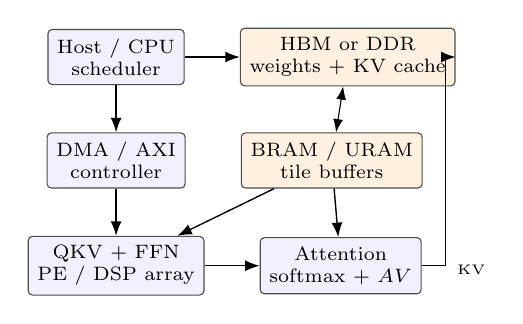
\begin{tikzpicture}[font=\scriptsize,>=Latex, node distance=3mm,
block/.style={draw=black!70,rounded corners=1.5pt,align=center,minimum height=6mm,fill=blue!6},
mem/.style={draw=black!70,rounded corners=1.5pt,align=center,minimum height=6mm,fill=orange!12},
arr/.style={->,line width=.5pt}]
\node[block,minimum width=1.5cm] (host) {Host / CPU\\scheduler};
\node[mem,right=7mm of host,minimum width=1.95cm] (hbm) {HBM or DDR\\weights + KV cache};
\node[block,below=6mm of host,minimum width=1.5cm] (dma) {DMA / AXI\\controller};
\node[mem,right=7mm of dma,minimum width=1.95cm] (buf) {BRAM / URAM\\tile buffers};
\node[block,below=6mm of dma,minimum width=1.5cm] (gemm) {QKV + FFN\\PE / DSP array};
\node[block,right=7mm of gemm,minimum width=1.95cm] (attn) {Attention\\softmax + $AV$};
\draw[arr] (host)--(hbm);
\draw[arr] (host)--(dma);
\draw[<->] (hbm)--(buf);
\draw[arr] (dma)--(gemm);
\draw[arr] (buf)--(gemm);
\draw[arr] (gemm)--(attn);
\draw[arr] (buf)--(attn);
\draw[arr] (attn.east) -- ++(3mm,0) |- (hbm.east);
\node[font=\tiny,anchor=west] at ($(attn.east)+(3.3mm,-.5mm)$) {KV};
\end{tikzpicture}
\caption{Conceptual CPU--FPGA decode datapath. The feedback path represents new KV writes and later KV reads. Buffer sizes, interfaces, and supported operators depend on the target device.}
\label{fig:arch}
\end{figure}

The design challenge is to balance the service rates of these stages. Aggressive loop unrolling can increase DSP demand without improving output rate if memory stalls dominate. Double buffering can overlap transfers and computation; systolic dataflow reduces repeated operand movement within a PE array. Conversely, softmax reductions, dynamic sequence lengths, scatter/gather cache access, and shape-dependent control can interrupt streaming. These limitations help explain why a high reported kernel throughput need not translate into high end-to-end token throughput \cite{blankestijn2026}.

\subsection{Published accelerator design patterns}
FTRANS showed an early approach to compressing Transformer matrices using block-circulant structure and mapping the resulting operations onto FPGA hardware \cite{li2020}. It primarily illustrates algorithm--architecture co-design rather than today's autoregressive LLM serving problem. FlightLLM addresses larger generative models with a configurable sparse DSP chain, an always-on-chip decoding approach, and a compilation strategy adaptive to sequence length. The authors report deployment on an Alveo U280 and comparisons with GPU baselines \cite{zeng2024}. EdgeLLM instead emphasizes a CPU--FPGA heterogeneous system, group-systolic processing, mixed-precision FP16$\times$INT4 and FP16$\times$FP16 arithmetic, structured sparsity, and end-to-end operator mapping on a VCU128 FPGA \cite{huang2025}.

At the other extreme, Chae and Kang describe an Artix-7 implementation that combines 4-bit quantization and MQA with an on-chip streaming Transformer design. They report 256-token cache support, post-synthesis throughput of 4.4 thousand tokens/s, 31.9\% BRAM utilization, and 85\% DSP utilization \cite{chae2025}. This is valuable evidence for compact fixed-function inference architectures, but the reported post-synthesis result must not be treated as a measured throughput of a general-purpose 7B LLM, nor directly ranked against larger systems' measured GPU baselines.

\subsection{HBM, DDR, and on-chip storage}
The attraction of HBM is high aggregate bandwidth delivered through multiple independently accessible channels. Bank placement, access concurrency, burst length, controller efficiency, and arbitration still determine whether an application approaches the rated bandwidth. DDR can offer substantial capacity at lower per-card bandwidth; BRAM and URAM offer fast local reuse but far smaller capacities. These roles are complementary, not interchangeable. Table~\ref{tab:memory} uses manufacturer specifications rather than measured LLM results.

\begin{table}[t]
\caption{Selected Memory Platforms: Vendor Specifications}
\label{tab:memory}
\centering
\footnotesize
\begin{tabular}{@{}p{1.1cm}p{2.05cm}p{3.75cm}@{}}
\toprule
Device & Memory & Stated capacity / bandwidth \\
\midrule
Alveo U280 \cite{amdU280} & HBM2; DDR4 & 8 GB / 460 GB/s aggregate HBM; 32 GB / 38 GB/s DDR \\
Kria KV260 \cite{amdKV260} & DDR4 (no HBM) & 4 GB DDR4; no directly comparable card-level bandwidth figure asserted here \\
A100 SXM 80 GB \cite{nvidiaA100} & HBM2e & 80 GB / 2039 GB/s rated bandwidth \\
\bottomrule
\end{tabular}
\end{table}

The U280's 460~GB/s HBM specification is much higher than its own 38~GB/s DDR specification but lower than the cited A100 SXM GPU specification. Thus ``HBM FPGA'' is not synonymous with ``more bandwidth than GPU.'' The U280's 8~GB HBM capacity cannot hold a raw 14~GB FP16 7B-parameter model entirely in HBM; low-bit compression, placement across HBM/DDR, or partitioning becomes necessary. Furthermore, a model fitting by raw weight size does not guarantee enough space for KV cache, workspace, buffers, or runtime bookkeeping \cite{amdU280,nvidiaA100}.

\subsection{Quantization and sparsity}
Quantization lowers weight traffic and can simplify FPGA arithmetic. SmoothQuant moves some activation-quantization difficulty into offline weight rescaling to enable W8A8 inference \cite{xiao2023}. Activation-aware weight quantization (AWQ) uses salience-aware scaling to preserve quality with low-bit weights \cite{lin2024}. A hardware team may exploit W4A16 matrix--vector units, INT8 dot-product packing, sparsity-aware skipping, and specialized nonlinear function approximations. Yet lower bit width may increase conversion or scaling overhead and requires task-appropriate quality validation. Unstructured sparsity is useful only if the representation and memory schedule avoid spending the savings on metadata and irregular accesses. FPGA flexibility is strongest when the selected model and encoding are known in advance; frequent model changes can undermine specialization benefits \cite{zeng2024,huang2025,blankestijn2026}.

\section{Comparative Evaluation: FPGA Versus GPU}
\subsection{Metrics and comparison protocol}
A credible comparison specifies (i) identical model architecture and quality target, (ii) numerical format and sparsity, (iii) prompt and generated-token lengths, (iv) batch size and concurrency, (v) warm-up and measurement interval, and (vi) whether the power figure covers the card or complete platform. \emph{Time to first token} (TTFT) includes prompt processing and relevant request overhead; \emph{inter-token latency} measures decode responsiveness; \emph{throughput} is sustained generated tokens per second. For a steady-state workload, energy per generated token is
\begin{equation}
E_{\mathrm{tok}}=\frac{P_{\mathrm{avg}}}{R_{\mathrm{tok}}}\quad [\mathrm{J/token}],
\label{eq:energy}
\end{equation}
where $P_{\mathrm{avg}}$ is the \emph{measured} average power under the stated system boundary and $R_{\mathrm{tok}}$ is generated tokens/s. This quotient needs careful interpretation if host energy, idle intervals, prefill, and decode are measured inconsistently. A thermal design power (TDP) rating is not an average runtime-power measurement.

\subsection{Published results and their comparability}
Table~\ref{tab:results} reports values from the cited works without combining their measurements into a common ranking. FlightLLM reports $6.0\times$ higher energy efficiency and $1.8\times$ better cost efficiency relative to tested GPU configurations including V100S for batch-one LLaMA2-7B; its separate VHK158 result reports $1.2\times$ higher throughput than an A100 baseline \cite{zeng2024}. EdgeLLM reports $1.91\times$ higher throughput and $7.55\times$ higher energy efficiency relative to the A100-SXM4-80G baseline in its IEEE journal version \cite{huang2025}. FTRANS reports up to $8.8\times$ improvement in energy efficiency over a GPU for its earlier Transformer workloads \cite{li2020}.

\begin{table*}[t]
\caption{Selected Reported FPGA Results (Author-Reported, Not a Unified Benchmark)}
\label{tab:results}
\centering
\footnotesize
\begin{tabular}{@{}p{1.65cm}p{2.45cm}p{2.45cm}p{3.0cm}p{5.2cm}@{}}
\toprule
Study & FPGA / workload & GPU comparator & Reported comparison & Interpretation and restriction \\
\midrule
FTRANS \cite{li2020} & FPGA Transformer compression and acceleration & GPUs in original study & Up to $8.8\times$ GPU energy efficiency & Earlier Transformer representations; not an apples-to-apples modern autoregressive LLM decode result. \\
FlightLLM \cite{zeng2024} & Alveo U280; LLaMA2-7B, batch one (reported setup) & V100S / other GPU baselines & $6.0\times$ energy efficiency; $1.8\times$ cost efficiency & Baseline software, compression, model and hardware all matter; figures are specific to reported setup. \\
FlightLLM \cite{zeng2024} & Versal VHK158 (separate result) & NVIDIA A100 & $1.2\times$ throughput & Different FPGA platform and comparison; not additive to the U280 improvement. \\
EdgeLLM \cite{huang2025} & VCU128 CPU--FPGA heterogeneous LLM implementation & NVIDIA A100-SXM4-80G & $1.91\times$ throughput; $7.55\times$ energy efficiency & Claimed in journal abstract; not directly comparable with FlightLLM's hardware or model conditions. \\
Chae--Kang \cite{chae2025} & Artix-7 compact quantized Transformer & No paired GPU benchmark & 4.4 k tokens/s \emph{post-synthesis} reported & No justified FPGA/GPU speedup; the throughput claim is not a measured deployment of a 7B LLM. \\
\bottomrule
\end{tabular}
\end{table*}

These results establish \emph{existence}, not universality, of favorable FPGA energy efficiency. No single study in the table reports a comprehensive comparison across all modern GPUs, batch sizes, model families, and context lengths. Nor do throughput gains necessarily imply proportional latency gains: deep batching can raise tokens/s while degrading a single user's TTFT or response latency. A claimed factor in tokens per joule corresponds to an inverse factor in joules per token only if the same token definition, workload and measurement boundary are maintained. Figure~\ref{fig:tradeoff} summarizes this interpretation.

\begin{figure}[t]
\centering
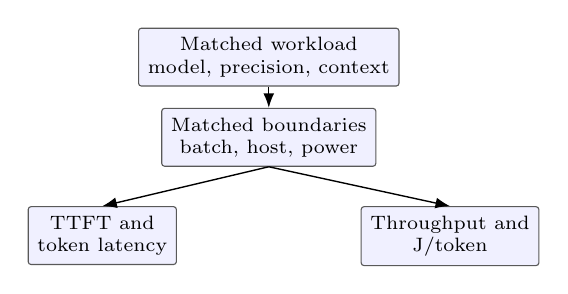
\begin{tikzpicture}[font=\scriptsize,>=Latex,
node distance=2.7mm,
bl/.style={draw=black!65,rounded corners=1pt,align=center,fill=blue!6,minimum height=6.2mm},
arrow/.style={->,line width=.5pt}]
\node[bl,minimum width=2.1cm] (work) {Matched workload\\model, precision, context};
\node[bl,below=of work,minimum width=2.1cm] (bound) {Matched boundaries\\batch, host, power};
\node[bl,below left=5mm and -2mm of bound,minimum width=1.5cm] (lat) {TTFT and\\token latency};
\node[bl,below right=5mm and -2mm of bound,minimum width=1.5cm] (energy) {Throughput and\\J/token};
\draw[arrow] (work)--(bound);
\draw[arrow] (bound.south)--(lat.north);
\draw[arrow] (bound.south)--(energy.north);
\end{tikzpicture}
\caption{Proposed minimum reporting framework for fair FPGA--GPU LLM inference comparison.}
\label{fig:tradeoff}
\end{figure}

\subsection{Critical limitations of available evidence}
Three issues limit generalization. First, the FPGA literature mixes encoder-style Transformers, compact bespoke decoders, and full autoregressive LLMs. Their computational intensity and cache pressure differ. Second, studies variously report estimated/post-synthesis outcomes, kernel timing, or full-system experiments. A clock-frequency estimate cannot replace a deployed energy-per-token measurement. Third, hardware generations and software stacks differ; a favorable comparison to V100S does not automatically transfer to A100 or newer GPU generations. The 2026 survey of Transformer deployment emphasizes similar benchmarking and disclosure problems \cite{blankestijn2026}.

Therefore, the most defensible interpretation of the reported FlightLLM and EdgeLLM figures is that \emph{specific co-designed FPGA systems can outperform specified GPU baselines under specified workloads}. A categorical statement that FPGAs are faster or more energy efficient than GPUs would not be supported. The decisive research contribution in an independent follow-up would be a controlled, reproducible experiment reporting absolute TTFT, decoding latency, generated tokens/s, peak memory occupancy, measured system watts, and joules per token at matched quality.

\subsection{Sensitivity of token metrics to serving conditions}
The apparent ranking of an accelerator can reverse as serving conditions change. During prefill, a long prompt increases the amount of attention computation and exposes many matrix--matrix operations; the relevant metric is often time to first token. During decoding, one token depends on the previous token, creating a sequential critical path, while the memory footprint of past K/V tensors increases with context length. Even when an attention engine performs dot products efficiently, longer contexts may force extra HBM traffic and reduce the token rate. This is precisely why an architecture optimized for a short fixed sequence should not be extrapolated to thousands of tokens without measurement \cite{shazeer2019,ainslie2023}.

Batching adds another trade-off. If many requests use the same weights in a shared execution window, effective weight reuse can raise arithmetic intensity and aggregate throughput. At the same time, (\ref{eq:kvcache}) shows that separate requests create additional KV state, making available memory and cache allocation increasingly important. PagedAttention addresses allocation efficiency, not the underlying capacity requirement \cite{kwon2023}. An FPGA implementation may therefore be advantageous for one latency target and disadvantageous for a different concurrency target. Reports should distinguish output tokens/s per \emph{request} from aggregate tokens/s across all requests.

Power accounting creates a separate source of disagreement. Equation~(\ref{eq:energy}) estimates steady-state energy per token from average power; for a finite request, a more faithful definition is the integral of power over the request interval divided by generated tokens. Whether prefill energy, host power, external DDR/HBM power, and idle recovery are included changes the answer. A low accelerator-die power figure does not necessarily imply low wall-plug energy per completed request. Equally, an energy-efficiency ratio cannot be converted into an absolute joules-per-token value when the original paper does not publish the relevant absolute power and token-rate figures.

Accordingly, the published table is interpreted as comparative \emph{evidence under individual study settings}, not as a meta-analysis with a common denominator. A reproducible follow-up benchmark should report at least three batch sizes, short and long prompts, fixed generated-token counts, cold and warm execution conditions, exact numeric precision, output quality, and both accelerator-only and complete-system power where instrumentation permits. These measurements would reveal which claimed advantage is due to hardware customization and which is due to workload selection or software-stack differences.

\section{Edge and Data-Center Feasibility}
\subsection{Edge devices: model fit before speed}
On an edge FPGA, low power, predictable latency, local data processing, and application-specific interfaces motivate hardware acceleration. Capacity imposes the first filter. For example, the AMD Kria KV260 provides 4~GB DDR4 but no HBM \cite{amdKV260}. Under the illustrative 7B model, the idealized 3.5~GB of 4-bit weights leaves little headroom for KV state, tensors, scales, operating system, and runtime. Consequently, a straightforward general-purpose 7B deployment on this kit would be highly constrained even before bandwidth and resource demands are considered. In contrast, a small quantized Transformer block, bounded-length attention engine, or fixed-task language model is a plausible research demonstrator; the Artix-7 study illustrates a related optimization direction \cite{chae2025}. Model quality must be assessed against the intended task, not merely against a resource-utilization target.

A tractable optional demonstration would prototype one attention or matrix--vector kernel in Vitis HLS, compare software and hardware output numerically, and measure latency for fixed sequence lengths. Such a study would test feasibility of \emph{a kernel}, not imply full LLM inference or superiority to a GPU. This distinction is particularly important when reusing an existing FPGA vision-processing toolchain: a CNN accelerator and a decoder-only Transformer exercise different compute, memory, and scheduling patterns.

\subsection{Data-center devices: HBM and utilization}
In data centers, throughput, multi-user concurrency, memory capacity, total cost, and measured energy dominate. HBM-equipped FPGAs can expose high external bandwidth while retaining specialized datapaths and adaptable precision. The value proposition is strongest for restricted model families, low- to moderate-batch inference, sparse or quantized weights, and deployments that can amortize compilation and integration costs \cite{zeng2024,huang2025}. Large contexts, concurrent sessions, and frequent model updates demand flexible cache management, sufficient capacity, and robust runtime scheduling. A GPU may be preferable where software support, model diversity, dynamic batching, and large aggregate HBM capacity outweigh FPGA customization.

For design teams, the appropriate decision procedure is: establish quality and context requirements; estimate parameter and KV memory; identify effective rather than rated bandwidth; choose precision and sparsity; model prefill/decode separately; then benchmark end-to-end latency and joules per token. The memory system must be designed together with the computation units. HBM alone cannot correct a poorly balanced pipeline or a stalled irregular access pattern.

\section{Conclusion}
FPGA inference efficiency arises from \emph{co-design}, not simply from placing a Transformer on programmable hardware. Autoregressive decoding couples repeated model-weight traffic with a growing KV cache; MQA/GQA, low-bit quantization, sparsity, and carefully scheduled on-chip buffers help relieve these constraints. HBM raises attainable memory bandwidth on suitable data-center devices but does not automatically exceed contemporary GPU bandwidth or solve capacity limits. Published FlightLLM and EdgeLLM studies report favorable results against selected GPU configurations, while FTRANS and compact on-chip demonstrations illustrate different workload classes and levels of evidence. The answer to the research question is therefore conditional: FPGAs can be competitive for specific, optimized inference regimes, but no general latency or energy advantage is established across all LLMs and GPUs. Future studies should standardize model quality, sequence lengths, batch sizes, power boundaries, and absolute token-level metrics so that architectural trade-offs can be assessed reproducibly.

\balance
\bibliographystyle{IEEEtran}
\bibliography{references}
\end{document}
